\section{Case Study\label{section:CS}}

\noindent
In this section\CV{,} we describe a realistic application of the system studied in this paper to perform surveillance operations. Considering the current COVID-19 restrictions, we focus on the problem of preventing and identifying possible concentrations of people during events such as popular or religious festivals. In particular\CV{,} we consider the Courtyards Festival of Cordoba (\url{https://patios.cordoba.es/es/}). This is a social event that takes place every year in the city of Cordoba, Spain, during the first two weeks of May. Courtyard’s owners decorate their houses with many flowers trying to win the award that is offered by the Town Hall. During this competition\CV{,} a festival runs in parallel with a number of artistic performances along six different paths located in different areas in the city as shown in Figure \ref{fig:mapPF}.
In the pandemic context, to monitor the situation to avoid \CV{the} concentration of people, we propose to apply a system consisting of one helicopter and a fleet of \LA{two} drones.
This kind of system has been proved successfully and has been already applied in the military field by the US Army to leave the helicopter at the edge of dangerous airspace and release drones, which will then penetrate \CV{the} enemy territory and send back intelligence, surveillance and reconnaissance information (see \cite{FGA}).
In our application\CV{,} the reason to adopt a similar system is the possibility to inspect simultaneously and in real time different paths\CV{,} also reducing the risk of flying the helicopter over populated areas and the cost of moving the helicopter by minimizing the total length of its tour.

\begin{figure}[h!]
\centering
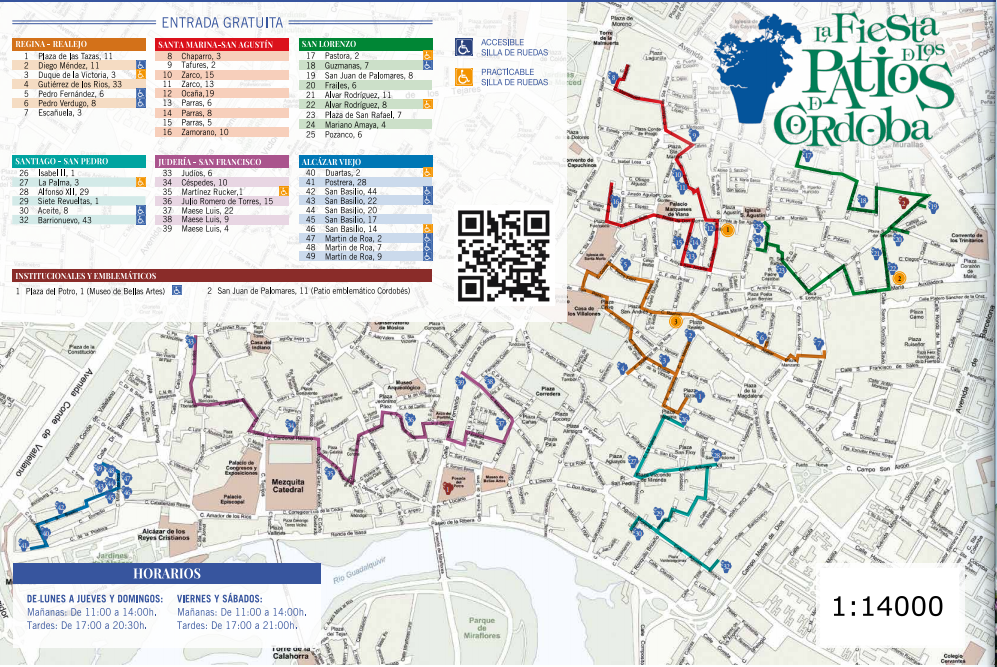
\includegraphics[width=0.6\linewidth]{figures/first.png}
\caption{Map of the Courtyards Festival in Cordoba. \label{fig:mapPF}}
\end{figure}

\noindent
We run the \LA{models} presented in Section \ref{Form} on this scenario starting from the initial solution provided by the matheuristic, where the 6 coloured paths reported in the map of Figure \ref{fig:mapPF} represent the 6 target graphs to be visited, in this case inspected, by the fleet of drones. In addition, we suppose that the drones' speed is \LA{43} km/h while that of the helicopter is  \LA{30} km/h aiming to minimize costs.
Moreover, we assume that the fleet is composed by \LA{two} drones with an endurance equal to \LA{7.5 minutes}, and we impose that each target graph must be fully visited (inspected).  As we can see from Figure \ref{fig:Mtour_CO} and Figure \ref{fig:Mtour_PO}, the origin of the mothership tour coincides with the destination and it is located in an area of the city where it is possible to assume the take-off and landing of an helicopter. Figure \ref{fig:Mtour_CO} reports the tour followed by the helicopter \LA{in} the solution \LA{of the complete overlapping version of the problem}, after \CV{4} hours of running time. We can observe that the helicopter, starting from the origin, flies to the point $x_R^1$ that is the first \LA{rendezvous} point, \LA{coinciding with the second launching point $x_L^2$}. Then, it flies along the edge connecting $x_R^1$ with $x_R^2$, that is the second rendezvous point, \LA{which coincides with the third launching point $x_L^3$}. Next, the helicopter flies to \LA{$x_R^3$ for retrieving the third drones' mission. From the same point the fourth and last mission starts and ends at point $x_R^4$, that is also the final destination of the helicopter tour.}\\
Figure \ref{fig:tourD_CO} shows the tour followed by the \LA{two} drones for inspecting the six paths. In particular, \LA{one drone, in red, starts from the origin ($origin=x_L^1$) for visiting the path of "Alcazar Viejo". It is retrieved by the helicopter at point $x_R^1$ and from the same point both drones, in red and blue, are launched to visit respectively the paths of "Juderia-San Francisco" and "Santa Maria-San Agustin". Both drones end their mission at point $x_R^2$. From this latter point they are launched to perform the visits to the paths of "San Lorenzo" and "Regina-Realejo". Then, they are both retrieved by the  helicopter at point $x_R^3$ where only one drone, the red one, starts its last mission to visit the path of "Santiago-San Pedro". In the meanwhile, the helicopter, containing the other drone (the blue one), flies to point $x_R^4=dest$ where it retrieves the red drone and ends its tour.}
The total time travelled by the helicopter is around 21 minutes.
\LA{We can observe that in the drone tour on "San Lorenzo" and "Regina-Realejo" graphs, there are two edges whose duplicate is represented with a dotted segment in Figure \ref{fig:tourD_CO}. They are associated with edges of the graph that are visited once, but travelled twice by the drone, in order to perform the inspection of the whole graph.\\
Figure \ref{fig:Mtour_PO} shows the mothership tour in the solution of the partial overlapping version of the problem, always obtained by setting a time limit of \CV{4} hours. In this case, we can observe that the helicopter follows a different tour and that there are more launching and retrieving points due to the possibility of launching a drone before retrieving the other one. From Figure \ref{fig:tourD_PO} we can see that, differently from the complete overlapping version, both drones start their first mission from the origin $origin=x_L^1=x_L^2$. The red drone visits the path of "Alcazar Viejo", while the blue one visits the path of "Santiago-San Pedro". The red drone is retrieved by the helicopter at point $x_R^3$ and it is launched again from the point $x_L^4$. From this latter point the red drone starts its second mission to visit the path of "Juderia-San Francisco". In the meantime, the helicopter flies to the point $x_R^5$ where the blue drone is retrieved. From the same point $x_R^5=x_L^6$ the blue drone is then launched to inspect the path of "Santa Maria-San Agustin". Both drones are retrieved by the helicopter at the point $x_R^7=x_R^8$ (shown in pink colour in Figure \ref{fig:tourD_PO}). From this latter point $x_R^8=x_L^9$ the red drone is launched to visit the path of "Regina-Realejo". Then, the helicopter flies to the point $x_L^{10}$ from where the blue drone starts its last visit to the path of "San Lorenzo". Finally, the helicopter flies to the destination $dest$ and along its path, it retrieves first the red drone at the point $x_R^{11}$ and then the blue one at the point $x_R^{12}$. Also in this case, like in the solution of the complete overlapping version of the problem, we have one edge of the graph associated with the path of "Regina-Realejo" and one edge of the graph representing the path of "San Lorenzo", that are traversed twice represented with dotted segments in Figure \ref{fig:tourD_PO}. The total travel time of the helicopter is 19 minutes. It is slightly lower than the one associated with the solution of the complete overlapping version of the problem. Thus, even if on this scenario we cannot observe big changes in terms of the objective function value, we can see how the different assumptions associated with the two versions of the problem can influence the structure of the solution, by producing a different schedule of the drone missions and a different location of the launching and rendezvous points.}\\
\noindent
All details of this case study, including map coordinates, .lp models and solutions can be found in \cite{Puerto2021}.


\begin{figure}[h!]
\centering
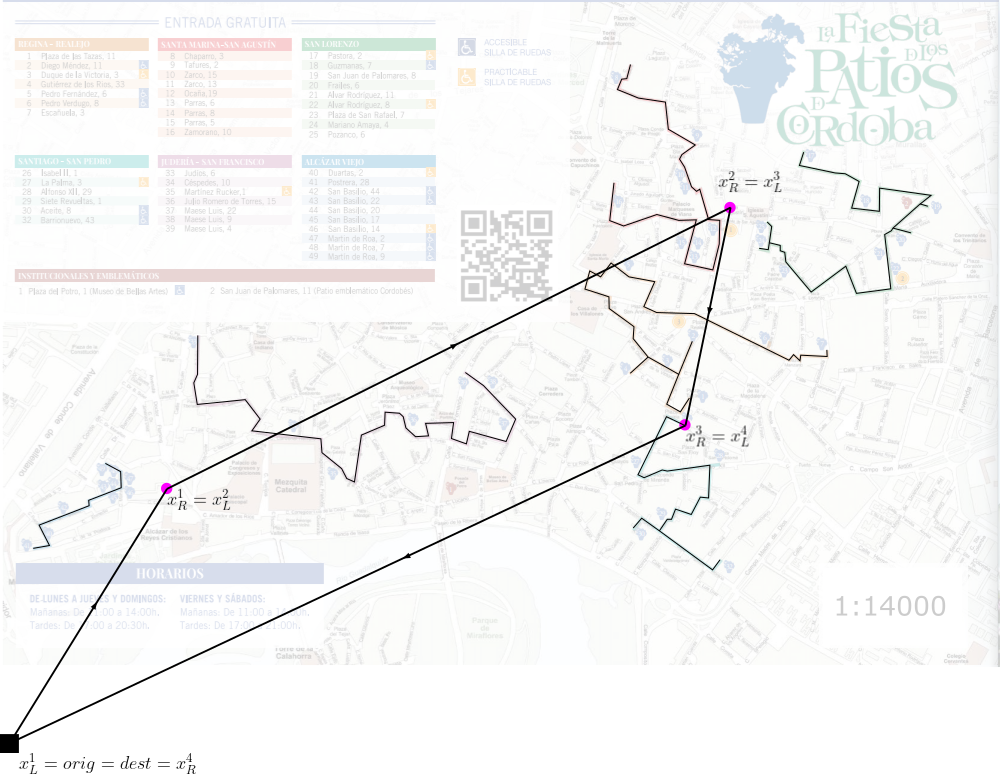
\includegraphics[width=0.6\linewidth]{figures/synchronous_1.png}
\caption{Mothership tour (CO) \label{fig:Mtour_CO}}
\end{figure}
\begin{figure}[h!]
\centering
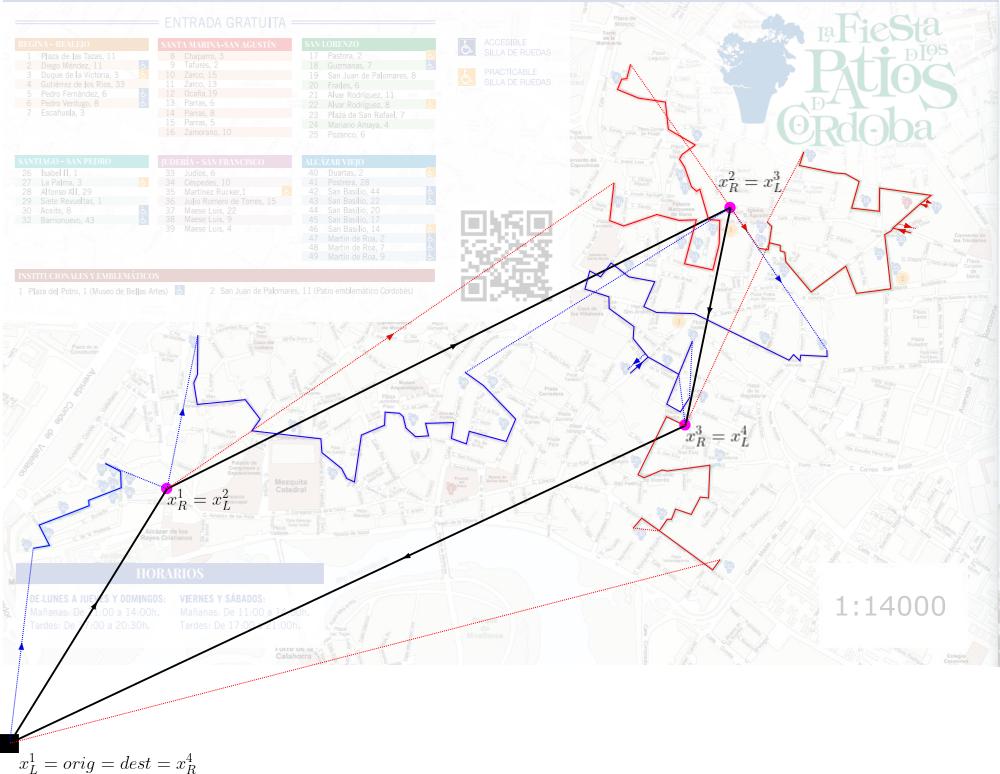
\includegraphics[width=0.6\linewidth]{figures/synchronous_2.png}
\caption{The complete solution (CO) \label{fig:tourD_CO}}
\end{figure}

\begin{figure}[h!]
\centering
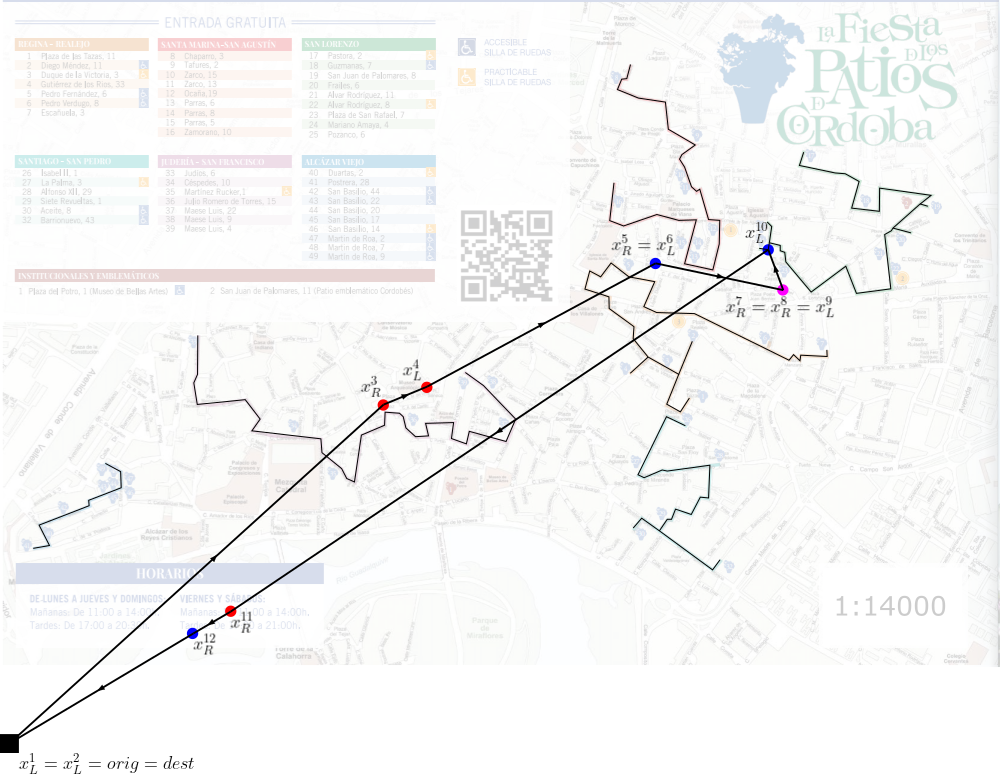
\includegraphics[width=0.6\linewidth]{figures/asynchronous_1.png}
\caption{Mothership tour (PO) \label{fig:Mtour_PO}}
\end{figure}
\begin{figure}[h!]
\centering
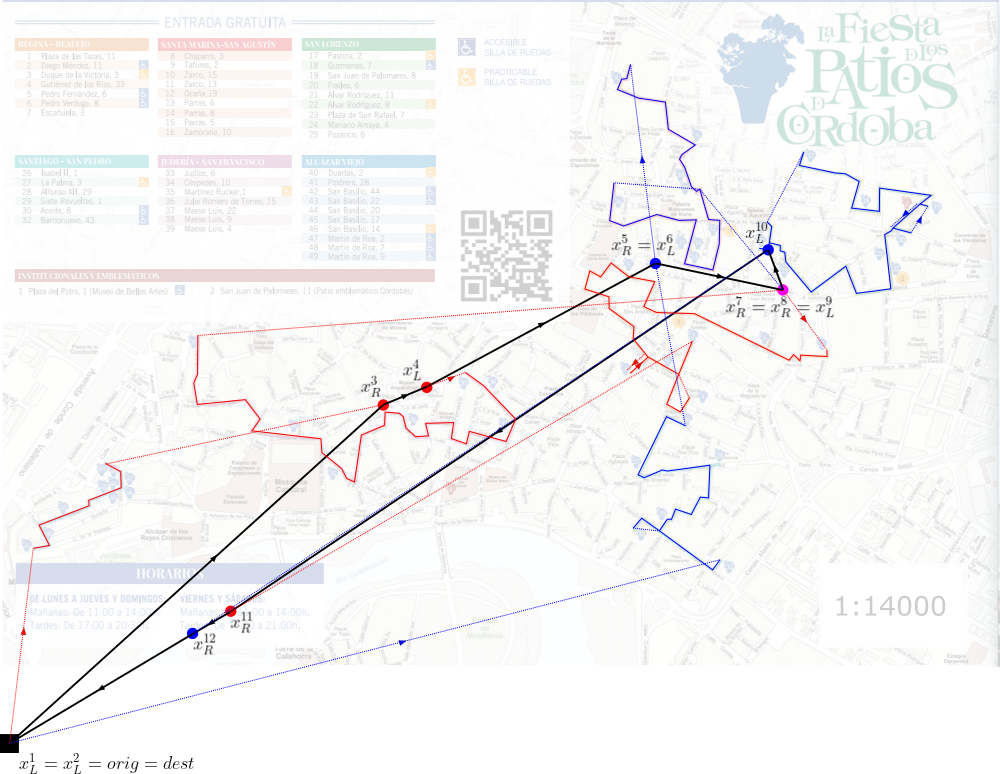
\includegraphics[width=0.6\linewidth]{figures/asynchronous_2.png}
\caption{The complete solution (PO) \label{fig:tourD_PO}}
\end{figure}